\section{Evaluation}\label{sec:evaluation}
\subsection{Descriptive seasonal analysis}
Table~\ref{tab:seasonal} describes the seasonal concentrations. Oxygen has its lowest mean in summer (7.040 mg/L) and its highest mean in winter (9.935 mg/L). Nitrate has its highest mean in summer (10.342 mg/L) and its lowest mean in winter (7.198 mg/L). Each season contains the same number of measurements from each river section.

\begin{table}[H]
\centering\small\singlespacing
\begin{tabular}{lrrr}
\toprule
Season & $n$ & Oxygen: mean (SD) & Nitrate: mean (SD) \\
\midrule
Spring & 225 & 9.531 (0.857) & 9.289 (2.591) \\
Summer & 225 & 7.040 (0.930) & 10.342 (2.744) \\
Autumn & 225 & 9.379 (0.888) & 8.418 (2.752) \\
Winter & 225 & 9.935 (0.779) & 7.198 (2.442) \\
\bottomrule
\end{tabular}

\caption{Seasonal mean and sample SD in mg/L, pooled over five sections.}\label{tab:seasonal}
\end{table}

Figure~\ref{fig:seasonal} shows the distributions. Spring and autumn oxygen overlap substantially. Their nitrate distributions also overlap, despite a larger difference in their means. Distributional overlap alone does not decide a test of mean differences; the inferential analysis evaluates uncertainty and multiplicity separately.

\begin{figure}[H]
\centering
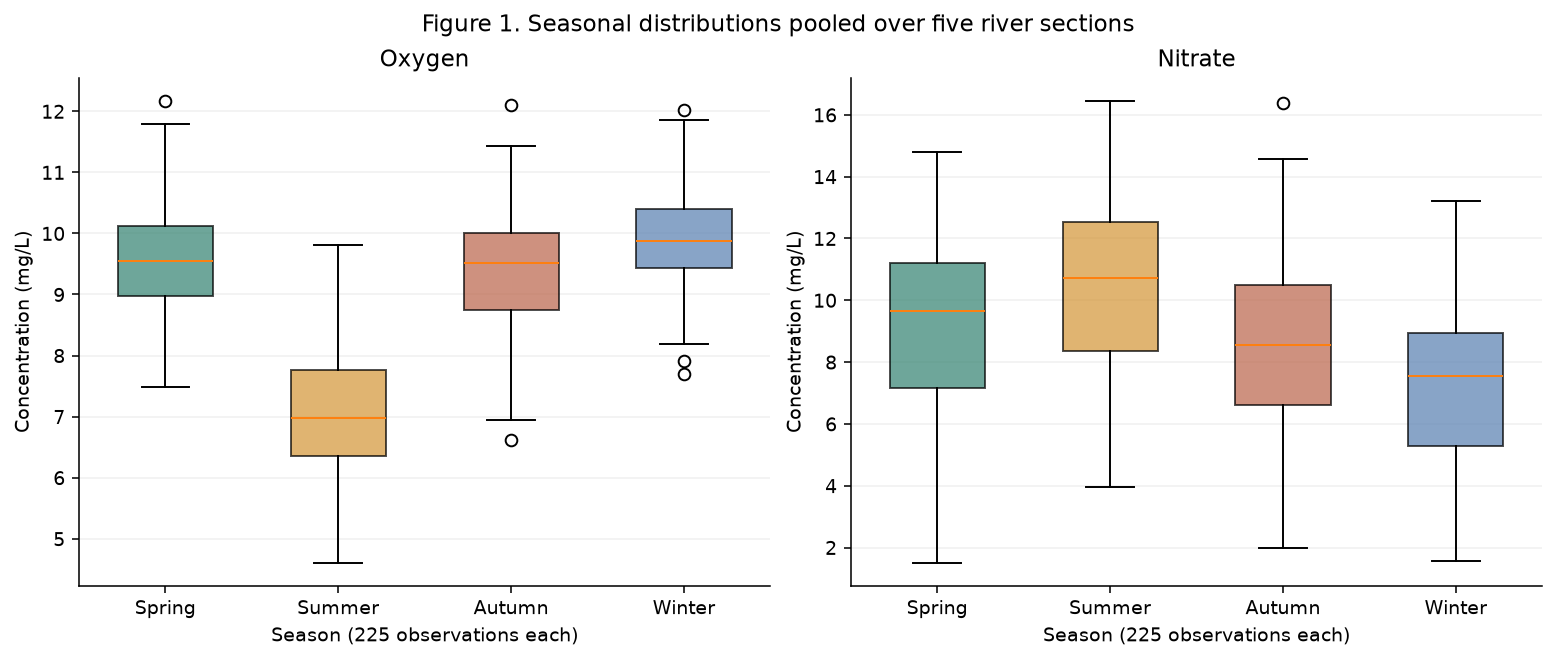
\includegraphics[width=\linewidth]{figures/seasonal_distributions.png}
\caption{Seasonal distributions, with 225 observations per season. Boxes mark the quartiles and median. Whiskers use the 1.5-IQR rule; points beyond them are retained observations.}\label{fig:seasonal}
\end{figure}

Spring oxygen has median 9.550 mg/L and IQR 1.153 mg/L; autumn oxygen has median 9.514 mg/L and IQR 1.265 mg/L. Spring nitrate has median 9.652 mg/L and IQR 4.039 mg/L; autumn nitrate has median 8.568 mg/L and IQR 3.883 mg/L. These location and dispersion summaries complement the means and SDs in Table~\ref{tab:seasonal}.
